\begin{landscape}
	\large
	\begin{center}
		\begin{tabular}{| l | l |}
			\hline\hline &  \\
			\multicolumn{1}{|c|}{\huge Translation} & \multicolumn{1}{c|}{\huge Rotation} \\
			& \\
			\hline
			\hline
			& \\
			Position $\vec s$ & Angle $\theta$ \\
			Velocity $\vec v$ & Angular velocity $\omega$ \\
			Acceleration $\vec a$ & Angular acceleration $\alpha$ \\
			& \\
			\hline
			\hline
			& \\
			$\vec s(t)=\frac{1}{2}\vec at^2 + \vec v_0 t + \vec s_0$ & $\theta(t) = \frac{1}{2}\alpha t^2 + \omega_0 t + \theta_0$ \\
			$\vec v(t)= \vec a t + \vec v_0$ & $\omega(t) = \alpha t + \omega_0$ \\

			& \\
			\hline
			\hline
			
			& \\
			Force $\vec F$ & Torque $\tau$ \\
			Mass $m$ & Rotational inertia $I$ \\
			Newton's second law $\vec F = m \vec a$ & Newton's second law for rotation $\tau = I \alpha$ \\
			& \\
			
			\hline
			\hline
			
			& \\
			Kinetic energy $KE=\frac{1}{2}mv^2$ & Kinetic energy $KE=\frac{1}{2}I\omega^2$ \\
			Work $W = \vec F \cdot \Delta \vec s$ & Work $W = \tau \Delta \theta$ \\
			Power $P = \vec F \cdot \vec v$ & Power $P = \tau \omega$ \\
			& \\
			
			\hline
			\hline
			
			& \\
			Momentum $\vec p = m \vec v$ & Angular momentum $L = I\omega$\\
			& \\
			
			\hline
						\hline
		\end{tabular}
	
	
	\bigskip
	
		``Rolling without slipping'' constraint: $v = \pm \omega r$ or $a = \pm \alpha r$
		
		\medskip
		
		(Think about the relative direction that the constraint imposes on $v$ and $\omega$ to determine whether the sign is $+$ or $-$)
	
	\end{center}
	
	
	\begin{center}

	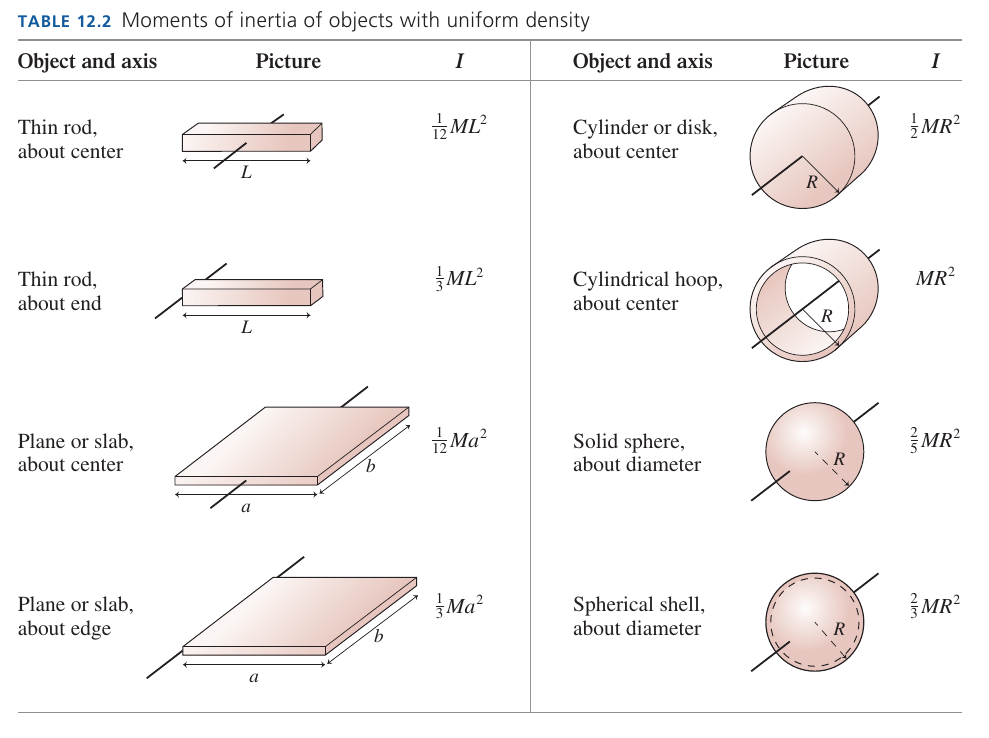
\includegraphics[width=7in]{moment-table.png}
	
	\Large
	
	In general, the moment of inertia is $I = \lambda MR^2$ or $I=\lambda ML^2$.
	
	\end{center}

\end{landscape}
